\documentclass[12pt,a4paper]{article}
\pagestyle{plain}
\usepackage{fullpage}
\usepackage[english]{babel}
\usepackage{enumerate}

%equations
\usepackage[fleqn]{amsmath}
\numberwithin{equation}{section}

%figures
\usepackage[dvips]{graphicx}
\graphicspath{{./images/}}
\numberwithin{figure}{section}

%excercises
\newcounter{Exercise}
\setcounter{Exercise}{1}
\usepackage[dvipsnames]{xcolor}
\usepackage{framed}
\definecolor{shadecolor}{gray}{0.9}
\usepackage{caption}

%tables
\numberwithin{table}{section}

%specials
\usepackage{textcomp} %special (greek) characters as text
%\usepackage{pstricks} %
%\usepackage{ifthen} %
%\usepackage{calc} %
%\usepackage{isotope}
\usepackage{hyperref}
\usepackage[bottom]{footmisc} %footnote below figure
\usepackage{footnpag}%number footnotes per page


%document details
\author{J. Kortland \\ translated and adapted by K. Schadenberg}
\date{}
\title{Early Research into Cosmic Radiation}


\begin{document}
\maketitle

\section{Introduction}
At the beginning of the 20th century physicists started to notice that charged objects slowly lost their charge, even when they were (almost) perfectly isolated. The behaviour of charge and charged object was investigated using a device designed around 1600, the electroscope. In this module we will take a look at how this instrument was used in the discovery of cosmic radiation.

\section{The Electroscope}
Most electroscopes have a similar design. Inside an isolated area (this can be free air in the simplest of designs) hangs a thin strip of sheet metal. This metal can be cheap aluminium but also more expensive gold. The strip of wire hangs from a conducting rod, also electrically isolated from the surroundings. Sometimes a large conducting plate or sphere is attached to the other end of this rod. Charging the electroscope can be done by bringing a charged object into contact with the metal rod, or the plate/sphere attached to the rod.

How does one charge an object? When the first electroscope was designed little was known about electricity, the battery was not even invented yet. The phenomenon of static electricity was known however. By rubbing two different materials together one could move charge from one material to another. Glass or ebonite rods are excellent materials to show this. Electroscopes were charged using this static electricity.

What happens when we charge an electroscope? Take a look at figure~\ref{fig:electroscope}, here we see a schematic representation of an electroscope being charged using an already charged rod. The two ends of the metal sheet now move away from each other.

\begin{figure}\begin{center}
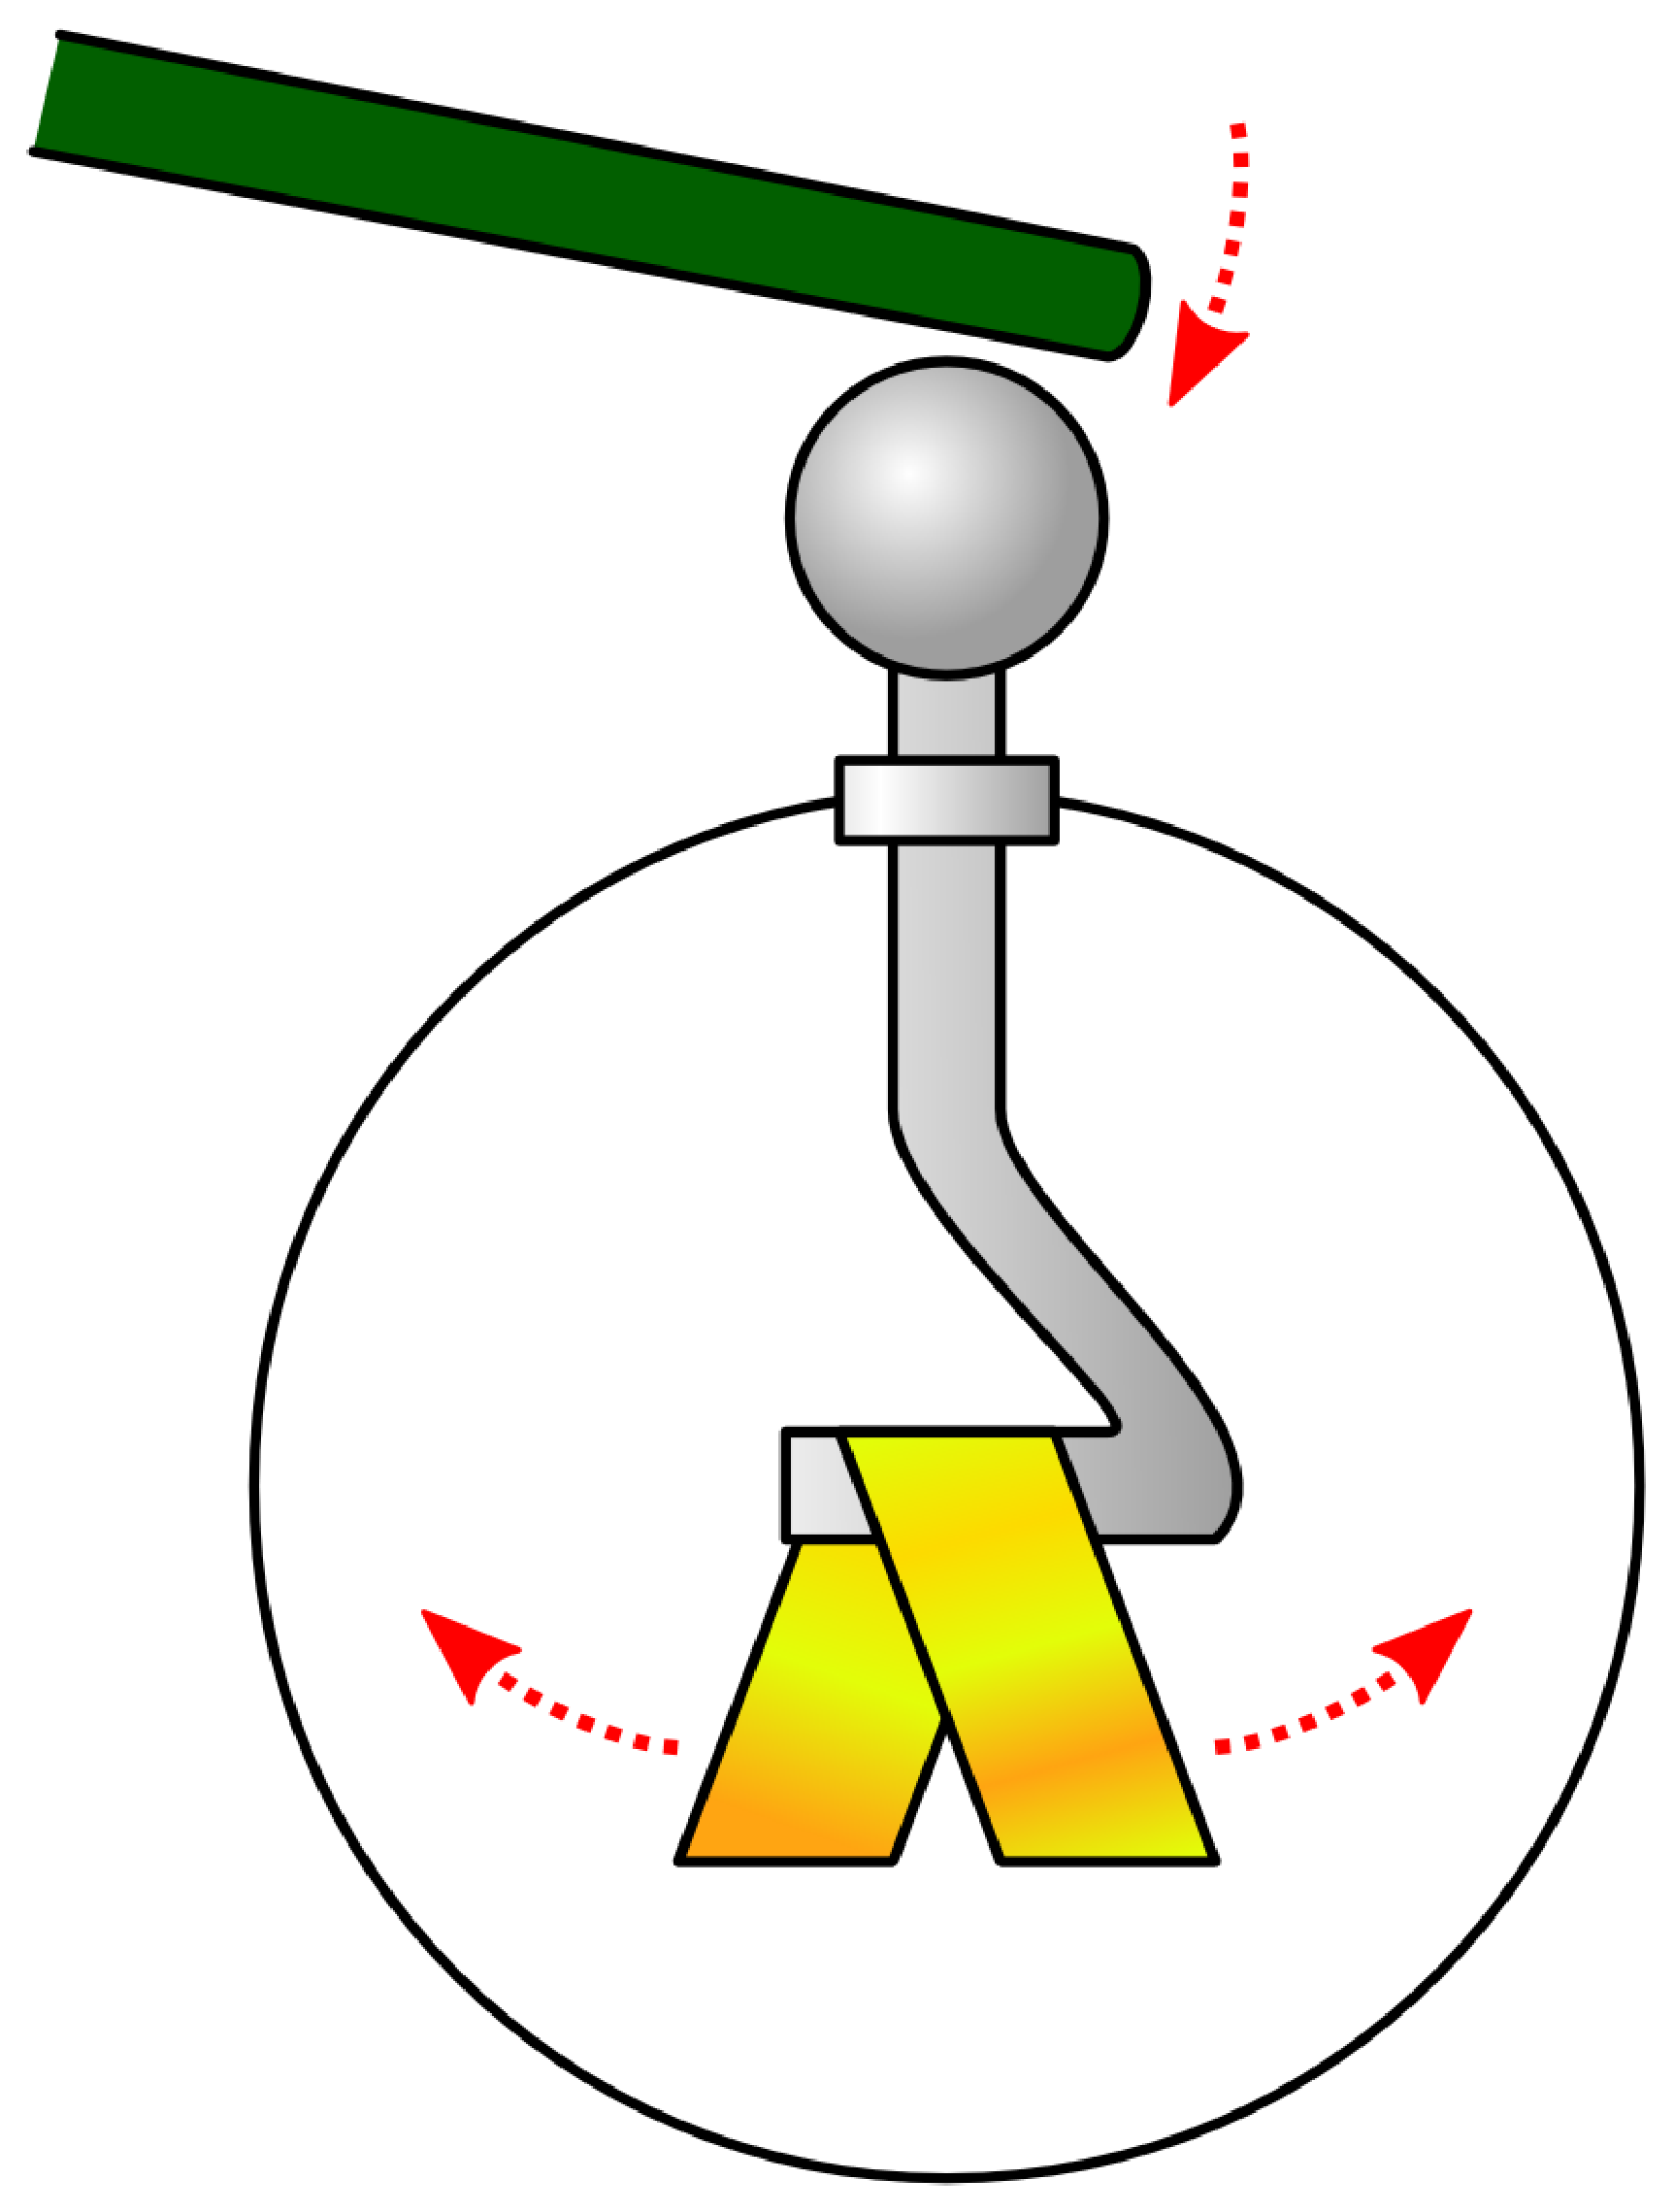
\includegraphics[scale=0.2]{Electroscope.eps}
\caption{A gold foil electroscope being charged by a nearby rod.\protect\footnotemark}\label{fig:electroscope}
\end{center}\end{figure}
\footnotetext{Picture taken from \url{http://en.wikipedia.org/wiki/File:Electroscope.png
}}

\begin{shaded}
\textbf{Exercise \theExercise \stepcounter{Exercise}} :
\begin{itemize}
\item[-] Why do the two ends of the metal sheet move away from each other?
\item[-] What is the connection between the size of the charge and the reading (distance between the two ends of the metal sheet) of the electroscope? Explain this connection.
\item[-] What will happen to the reading of the electroscope when the charge slowly leaks away?
\item[-] A charged electroscope will discharge near a flame or radioactive source. Explain why this happens.
\end{itemize}\end{shaded}

\subsection{Research into Radioactivity}
At the start of the 20th century three now famous scientists, Henri Becquerel, Marie Curie-Sklodowska, and Pierre Curie, were researching different radioactive salts. Their findings gave an answer to the mystery of the discharging electroscopes. Radioactive radiation can ionise air. The air which should function as an isolator in an electroscope can thus become slightly conducting, letting the charge leak away.

Isolating the different origins of this radioactive radiation was however a bit more difficult. From the research into uranium salts it was known that there are different sources of radiation in the Earth's crust. Further research showed that there were also sources of radioactivity in the seas and the atmosphere, all of them capable of discharging an electroscope. However, during this research an interesting phenomenon was observed. Using lead to shield the electroscope slowed down the rate of discharge but could never completely stop it, however thick the layers of lead where made.

\subsection{Finding the Sources of Radiation}
This meant that there had to be a very powerful and yet unknown type and source of radiation capable of penetrating thick sheets of lead. Finding this source of radiation was not the work of just one man. But Victor F. Hess was the first to make some important breakthroughs and show that this source must be cosmic in origin. For his work he was awarded the Nobel Prize in Physics in 1936.

\begin{figure}\begin{center}
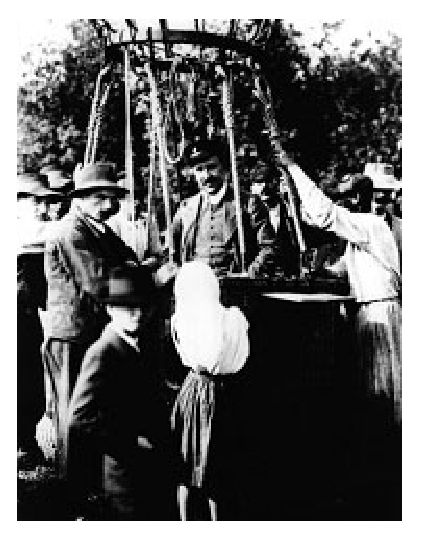
\includegraphics[scale=1]{Hess.eps}
\caption{Victor Hess just before his famous balloon flight.}\label{fig:hess}
\end{center}\end{figure}

\begin{shaded}
\textbf{Exercise \theExercise \stepcounter{Exercise}} : The working theory when trying to find the source of radiation that discharged electroscopes was that the source must be somewhere inside the Earth's crust.
\begin{itemize}
\item[-] In 1910 Theodor Wulf took his electroscope to the top of the Eiffel Tower, at 300 metres the tallest building at that time. Here his electroscope discharged at a slower rate than at the base of the tower. What must have been his conclusion?
\item[-] In 1911 and 1912 Victor Hess made a few balloon flights. During which he saw that at first, with an increase in height the rate of discharge decreased, but at high altitudes the rate of discharge greatly increased. What must have been his conclusion? 
\item[-] How would you design an experiment to test whether the radiation comes from the Sun or not?
\item[-] Below is a part of the Nobel Lecture of Victor Hess, use this text to 	check your previous answers.

\textit{When, in 1912, I was able to demonstrate by means of a series of balloon ascents, that the ionization in a hermetically sealed vessel was reduced with increasing height from the earth (reduction in the effect of radioactive substances in the earth), but that it noticeably increased from 1,000~m onwards, and at 5~km height reached several times the observed value at earth level, I concluded that this ionisation might be attributed to the penetration of the earth's atmosphere from outer space by hitherto unknown radiation of exceptionally high penetrating capacity, which was still able to ionize the air at the earth's surface noticeably. \\
Already at that time I sought to clarify the origin of this radiation, for which purpose I undertook a balloon ascent at the time of a nearly complete solar eclipse on the 12th April 1912, and took measurements at heights of two to three kilometres. As I was able to observe no reduction in ionisation during the eclipse I decided that, essentially, the sun could not be the source of cosmic rays, at least as far as undeflected rays were concerned.}
\end{itemize} \end{shaded}

The conclusion of Hess and others was that the unknown radiation can from (outer) space, this led to the naming of cosmic radiation and cosmic rays.

You can redo Hess his experiment using an online applet at: \\
\url{http://sunshine.chpc.utah.edu/javalabs/java102/hess/balloon/index.htm}

\begin{shaded}
\textbf{Exercise \theExercise \stepcounter{Exercise}} : Research into cosmic radiation only started with its discovery. In 1920 Jacob Clay tried to measure the variation in cosmic ray intensity with latitude. During his boat trips to and from Indonesia he notices that the intensity decreases when travelling from a high latitude towards the equator.\\
What clue does this observation give us into the nature of cosmic radiation? \end{shaded}

\section{History of Science}
The text above only scratches the surface of the story of the discovery of cosmic radiation. The entire history spans from roughly 1785 to the middle of the 1930s. A large number of (now famous) physicists were involved in this story, sometimes with opposing views or opinions. Their quest for answers, the way they performed their research, and engaged in debate with one another trying to convince their `opponents', is really a story about the scientific process. The following text, at the moment only available in Dutch, goes a little deeper into this subject and contains further questions and assignments:\\
Hans Leppink (2004), \textit{De ontdekking van de oorsprong van kosmische straling.} Amsterdam: Vrije Universiteit

\section{Elementary Particles}
With the discovery of cosmic radiation, particle physics could advance a little further. Researchers now had at their disposal a large particle accelerator to look for new particles. With cosmic radiation the first of new exiting particles were discovered: muons, pions, and  positrons. The simple view of only protons, neutrons, and electrons had to be revised. 

Most of these new particles turned out to be unstable. This and other discoveries only led to more questions such as `Are there positive muons?' and `Why is the electron stable but the muon unstable?'. Researchers had to wait until the 1960 for particle accelerators and colliders which were powerful enough to answer these and other questions. When these became available most particle physicists left cosmic rays behind to work with colliders. The advantages were very clear. Although cosmic radiation was always and freely available, it could not be controlled. Getting your experimental equipment in the right place at the right time was difficult, time intensive, and costly. Building a particle accelerator might be difficult, but obtaining measurements and analysing them was much easier.


\end{document}


\begin{shaded}
\textbf{Exercise \theExercise \stepcounter{Exercise}} : \end{shaded}

\footnotemark
\footnotetext{}

\begin{figure}\begin{center}
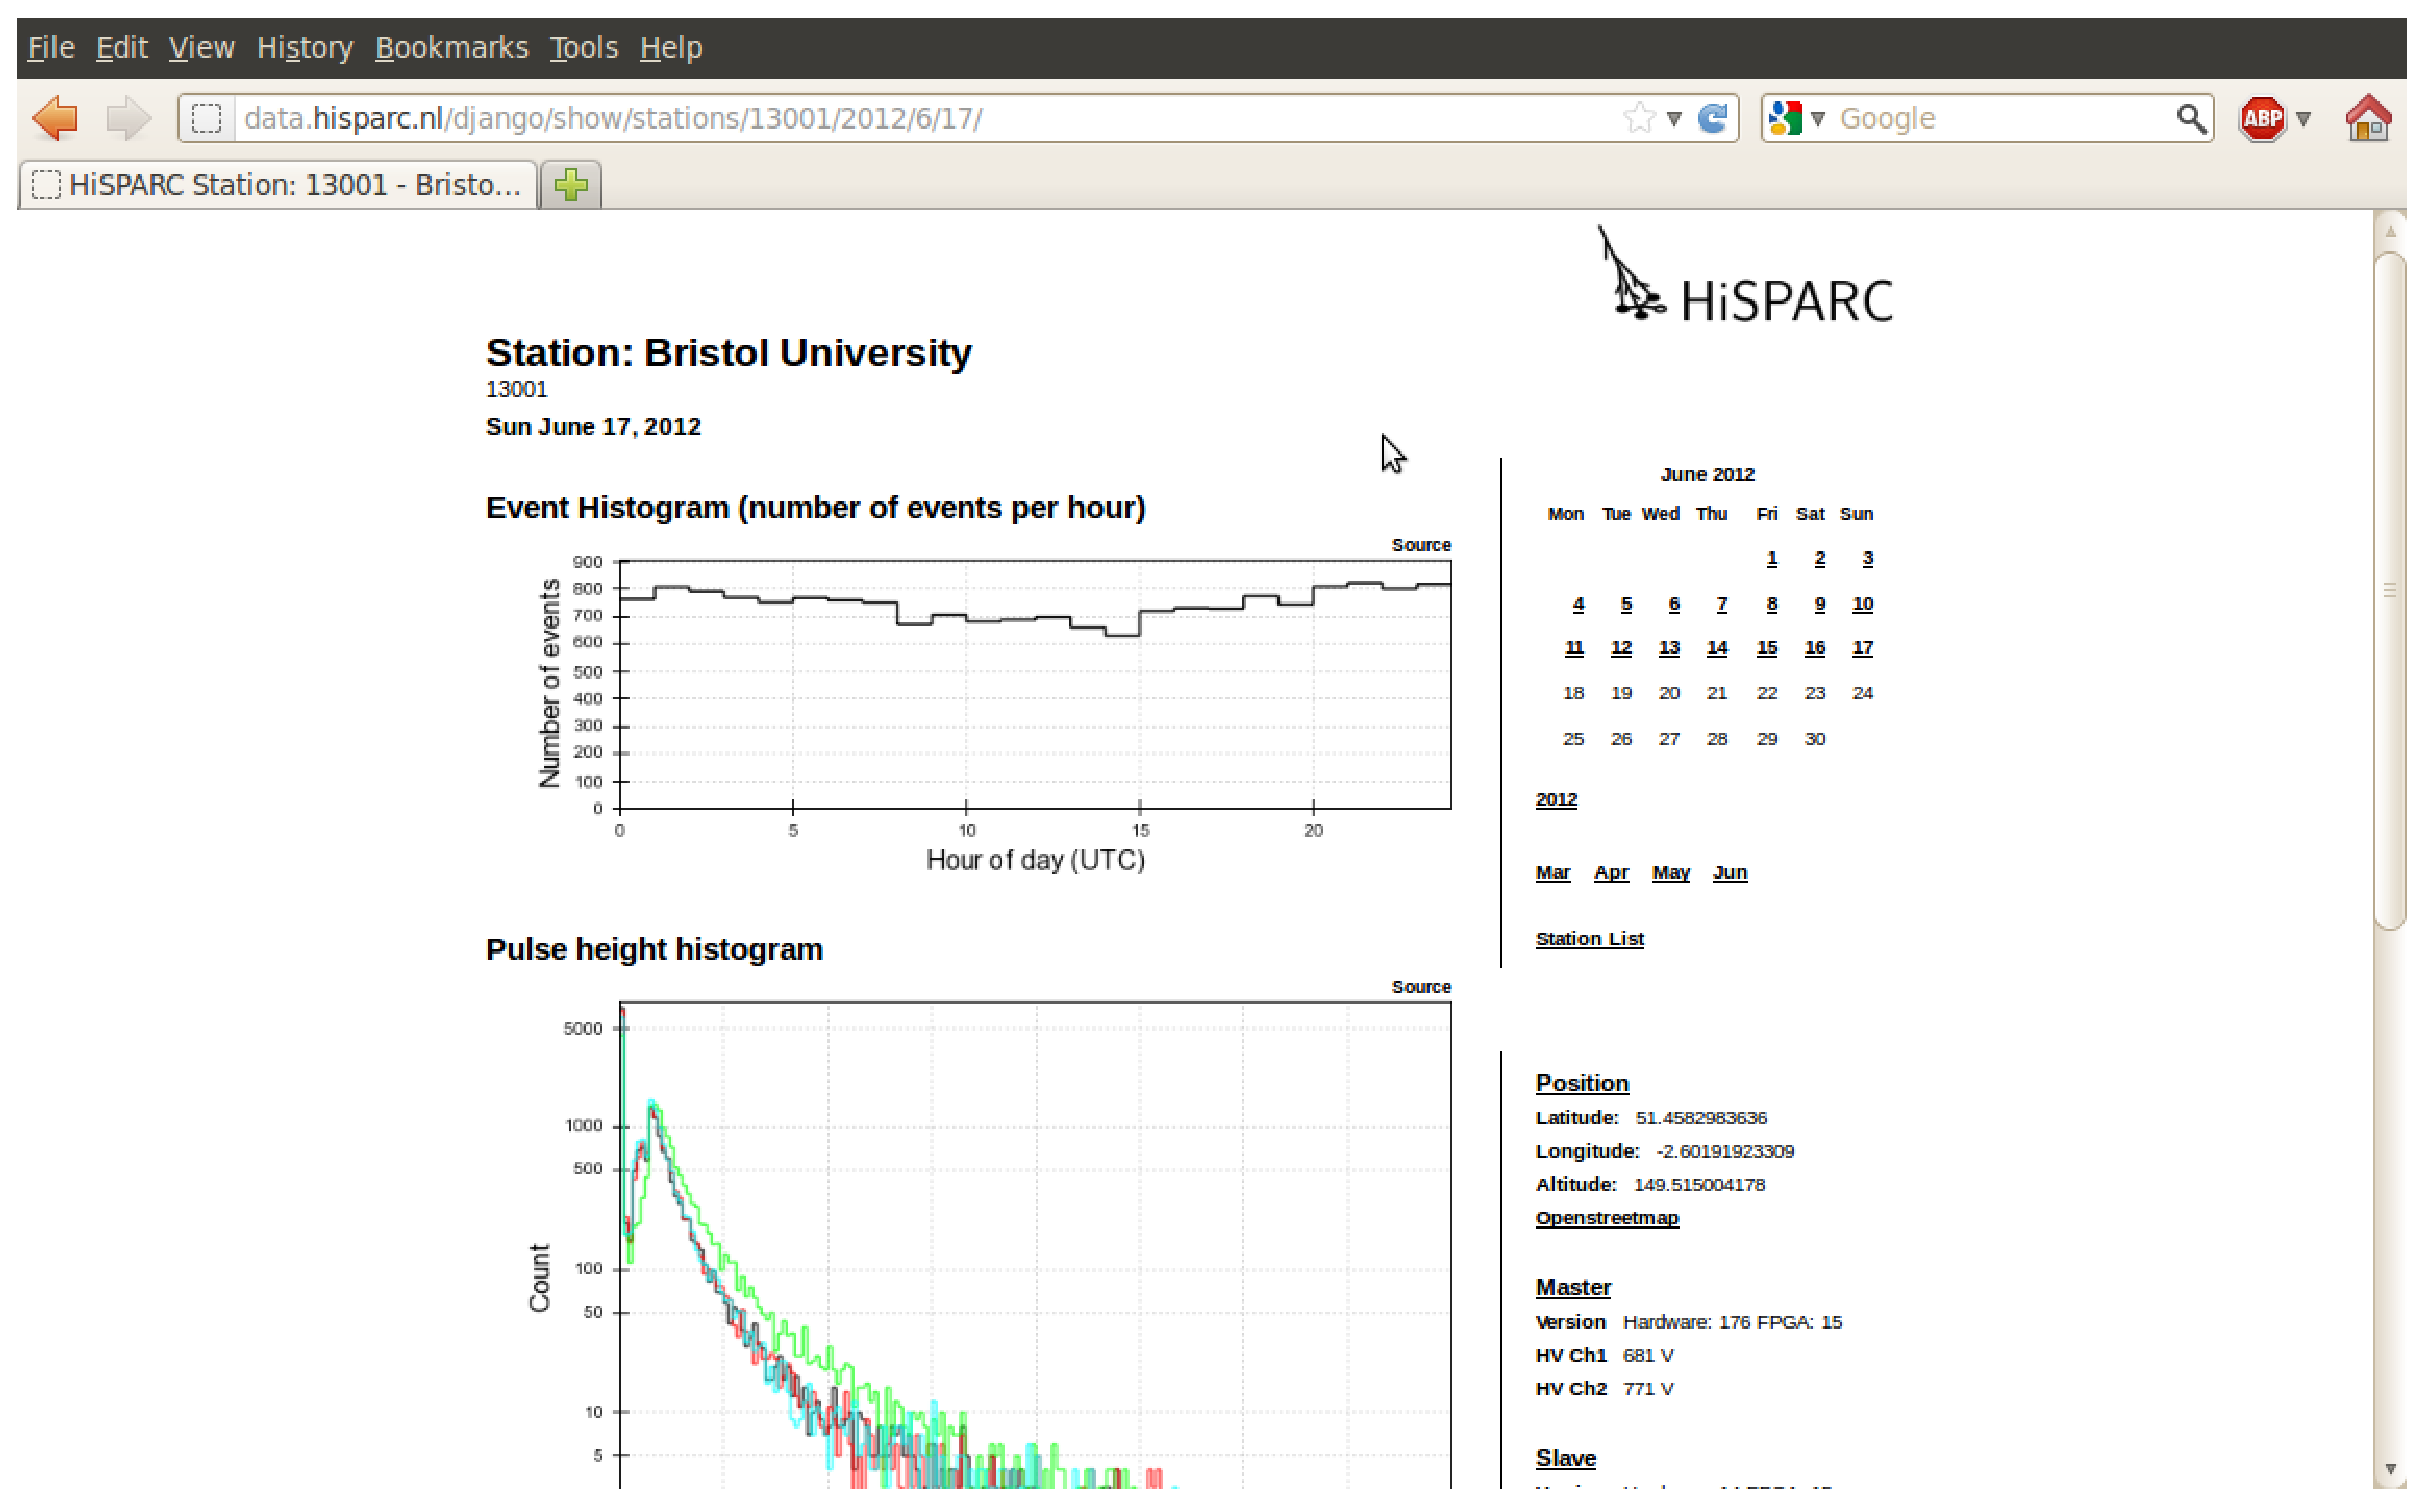
\includegraphics[scale=0.3]{Screenshot_HiSPARC_Station_13001.eps}
\caption{Information available via \protect\url{http://data.hisparc.nl/} .}\label{fig:data_screen}
\end{center}\end{figure}
